\chapter{confelm}

\section{Introduction}
One way in which information about confluence can be used before state space generation, is by appending confluent ISTEPs to other summands.
This has the effect that other branches that could follow those summands are ignored, reducing the size of the state space while maintaining its equivalence up to branching bisimulation.

\section{Formal background}

\subsection{Definite successors}

Consider a summand pair $(s_\alpha, s_\beta)$, referencing the elements of $s_\alpha$ and $s_\beta$ conform \ref{summandelements}.
Summand $s_\beta$ is said to be a \emph{definite successor} of $s_\alpha$ if the following expression is a tautology:
\begin{align*}
g_\alpha \rightarrow {g_\beta}[v \mapsto q(v) \;|\; v \in \varsof{g_\beta} \setminus P][p \mapsto v_\alpha(p) \;|\; p \in P]
\end{align*}

where $q(v)$ is a bijective function that relates variable $v$ to a fresh variable.

For a summand $s$, let $D(s)$ be the set of all definite successors of $s$.
By design, $D(s)$ is an under-approximation of the actual successors of $s$.

\section{Algorithm}

The algorithm follows these steps:

\begin{enumerate}

\item Determine which \istep{} summands of the LPE are confluent (see \ref{confcheck}).
Rename the \istep{} channels in confluent \istep{} summands to \cistep{}.

\item For each summand $s_\alpha$, determine $D(s_\alpha)$.
Consider all possible pairs of summands $(s_\alpha, s_\beta)$ such that $s_\beta \in D(s_\alpha)$ and $C_\beta = \cistep{}$, and reference the elements of $s_\alpha$ and $s_\beta$ conform \ref{summandelements}.

Let
\begin{align*}
X = [ x_\beta(j) \mapsto q(x_\beta(j)) \;|\; 1 \leq j \leq m_\beta ]
\end{align*}

where $q(x)$ is a surjective function that yields fresh variables, and let
\begin{align*}
V_\alpha &= [p_j \mapsto v_\alpha(p_j) \;|\; 1 \leq j \leq k]
\end{align*}

Replace $s_\alpha$ by ${s_\alpha}'$, which is defined as
\begin{align*}
{s_\alpha}' = C_\alpha \; &\texttt{?} \; x_\alpha(1) \; \cdots{} \; \texttt{?} \; x_\alpha(m_\alpha) \\
&\texttt{?} \; x_\beta(1)[X] \; \cdots{} \; \texttt{?} \; x_\beta(m_\beta)[X] \\
&[[g_\alpha]] \; \texttt{>->} \; P(v_\beta(p_1)[X][V_1], \cdots{}, v_2(p_k)[X][V_\alpha])
\end{align*}

\item Replace all occurrences of \cistep{} channels with \istep{} channels.
\end{enumerate}

\section{Example}

Consider the following example:

\begin{lstlisting}
//Process definition:
PROCDEF example[A :: Int](x, y :: Int)
  = A >-> example[A]((x+1) mod 3, y)
  + CISTEP >-> example[A](x, (y+1) mod 4)
  ;

//Initialization:
example[A](0, 0);
\end{lstlisting}

The second summand is a \cistep{} summand.
It is also a definite successor of the first summand.
This means that the second summand will be appended to the first summand.

The second summand is also a definite successor of itself.
This means that the second summand will also be appended to itself.

Therefore, the original process is changed to

\begin{lstlisting}
//Process definition:
PROCDEF example[A :: Int](x, y :: Int)
  = A >-> example[A]((x+1) mod 3, (y+1) mod 4)
  + ISTEP >-> example[A](x, (((y+1) mod 4)+1) mod 4)
  ;

//Initialization:
example[A](0, 0);
\end{lstlisting}

\section{Benchmark results TODO}

TODO

\begin{figure}[!ht]
\begin{center}
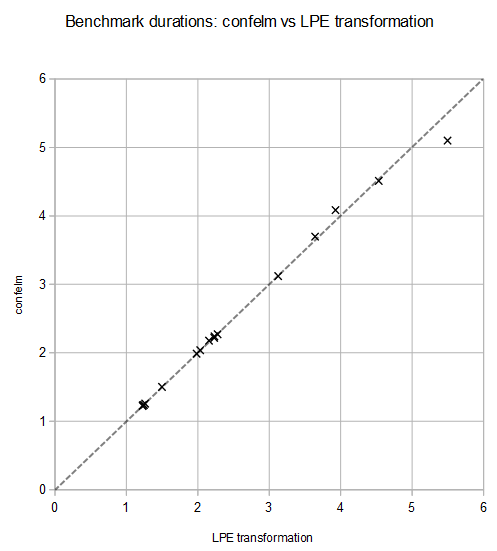
\includegraphics[width=0.7\linewidth]{charts/confelm-vs-lpe-only}
\caption{Benchmark results: confelm vs LPE transformation}
\label{confelm-vs-lpe-only:fig}
\end{center}
\end{figure}


